\section{Evaluation}

\subsection{Research Questions}

The evaluation follows the dependencies of the released detector. \textbf{RQ1} asks whether one frozen \method{} checkpoint is effective relative to no-fit controls, official forecasting-foundation checkpoints, and the broader TShape baseline ledger. \textbf{RQ2} measures how Pattern Bank size changes optimization and EasyTSAD F1 on each target. \textbf{RQ3} isolates the failures repaired by the Residual Guard and the marginal value that remains attributable to TShape. \textbf{RQ4} examines the effectiveness--footprint tradeoff and the learned attention behavior on a real incident. All questions use the same two metrics defined in Section~II-A.

\subsection{Experimental Setup}

\begin{table}[t]
\caption{Full-coverage benchmark families. ``Ano.'' is the median anomalous-point ratio per series.}
\label{tab:data}
\centering
\scriptsize
\setlength{\tabcolsep}{3.2pt}
\begin{tabular}{lrrrr}
\toprule
Dataset & Series & Test points & Med. length & Med. ano. \\
\midrule
AIOPS & 29 & 3,073,556 & 131,795 & 1.269\% \\
NAB & 10 & 79,318 & 7,928 & 6.581\% \\
TODS & 15 & 75,000 & 5,000 & 5.360\% \\
UCR & 203 & 7,782,539 & 22,826 & 0.643\% \\
WSD & 210 & 3,829,537 & 18,236 & 0.310\% \\
Yahoo & 367 & 286,559 & 840 & 0.422\% \\
\midrule
Total & 834 & 15,126,509 & -- & -- \\
\bottomrule
\end{tabular}
\end{table}

\textbf{Datasets.}
Table~\ref{tab:data} contains 15.1 million observations from six distinct families. AIOPS comprises production KPIs from large Internet services, while WSD contains high-frequency Web-service KPIs; both directly represent software operations. NAB includes real streaming cloud, traffic, advertisement, and server-like signals~\cite{ahmad2017nab}. UCR contributes heterogeneous expert-labeled rare events, TODS contributes controlled anomaly variation, and Yahoo contributes real and synthetic Webscope streams. The original TShape study reports the first five; Yahoo is an artifact extension. The shared first-difference contract consumes one warm-up point per series, leaving 15,125,675 scored points. UCR, WSD, and Yahoo contain 2, 49, and 15 all-normal test series. They remain in coverage and resource totals but cannot define F1.

\textbf{Methods and access contracts.}
The public ledger contains 44 executable configurations and records whether each row is a no-fit control, released frozen checkpoint, strict synthetic-only checkpoint, source adaptation, family adapter, target-context diagnostic, or ablation. Table~\ref{tab:all-easytsad} omits the five residual controls and its Access column to keep the dense six-dataset comparison readable; their results remain available in the ledger and are analyzed explicitly in RQ3. Red/blue ranking in the table is restricted to released frozen foundation checkpoints and our strict synthetic-only checkpoints. This distinction remains essential: an adapter tests a scoring family under the common interface but is not represented as the original authors' checkpoint.

The residual controls are persistence, rolling mean, rolling median, spectral residual, and rolling MAD. The frozen-checkpoint group executes Chronos-Bolt-Tiny, Timer-base-84M, TimesFM-2.5-200M, and Sundial-base-128M directly; their preceding-context forecasts are converted to squared residual scores. Context/horizon pairs are 64/64, 384/96, 384/96, and 720/720. Official TimeMoE-50M exceeded the predeclared ten-minute optional-checkpoint screen and is not reported partially. A separately identified TimeMoE family adapter remains in the table. The ledger also retains every family represented in the original TShape comparison, including SubLOF, SAND, Matrix Profile, AR, LSTMAD, AE, EncDecAD, SRCNN, Anomaly Transformer, TFAD, TranAD, Donut, FCVAE, TimesNet, OFA, FITS, and KAN-AD.

\textbf{Execution and statistics.}
Every included method scores 834/834 series. All experiments use seed 20260704 on an 8-core Apple M3 with 16~GB unified memory. TShape uses PyTorch 2.0.0 with MPS, training batch 256, evaluation batch 2,048, and dense stride-one inference. The final Pattern checkpoint trains on all 60,000 generated windows with Adam, a maximum of 30 epochs, and patience-three early stopping. Labels are opened only after each score stream is frozen. For \method{} minus a comparator, the analysis unit is a series. We report mean paired difference and a 10,000-resample percentile bootstrap 95\% interval, together with wins, losses, ties, and an exact two-sided sign test in the artifact. These intervals measure cross-series heterogeneity under the fixed run; one seed does not establish training-seed stability.

The optimized metric adapter was checked against EasyTSAD 0.3.0.2 on 16 boundary traces and 200 randomized traces, including terminal events, tied scores, all-normal inputs, single-point events, and varying event lengths. \pfone{}, \efone{}, precision, recall, and selected thresholds matched exactly. Every result row exposes valid-series counts and coverage.

\subsection{RQ1: Overall Performance}

\begin{table*}[t]
\centering
\caption{Full-coverage non-residual comparison under one EasyTSAD protocol (Point-F1 / Event-F1). Among official frozen foundation checkpoints and strict synthetic-only TShape checkpoints, \textcolor{red}{red bold} and \textcolor{blue}{blue underlined} mark the best and second-best score per metric. Adapter, adaptation, diagnostic, and ablation provenance is retained in the public result ledger.}
\label{tab:all-easytsad}
\scriptsize
\setlength{\tabcolsep}{2.8pt}
\renewcommand{\arraystretch}{0.91}
\resizebox{\textwidth}{!}{%
\begin{tabular}{@{}llcccccc@{}}
\toprule
Family & Method & AIOPS & NAB & TODS & UCR & WSD & Yahoo \\
\midrule
Foundation & Chronos-Bolt-Tiny & 0.889 / 0.786 & 0.998 / 0.881 & 0.646 / 0.521 & 0.628 / 0.324 & 0.969 / 0.893 & \textcolor{blue}{\underline{0.762}} / \textcolor{blue}{\underline{0.739}} \\
 & Timer-base-84M & 0.886 / 0.781 & 0.990 / 0.862 & 0.752 / 0.615 & \textcolor{blue}{\underline{0.689}} / \textcolor{red}{\textbf{0.410}} & 0.963 / 0.890 & 0.731 / 0.699 \\
 & TimesFM-2.5-200M & \textcolor{red}{\textbf{0.896}} / \textcolor{red}{\textbf{0.800}} & 0.997 / 0.875 & \textcolor{red}{\textbf{0.818}} / \textcolor{red}{\textbf{0.688}} & \textcolor{red}{\textbf{0.705}} / \textcolor{blue}{\underline{0.399}} & \textcolor{red}{\textbf{0.971}} / \textcolor{red}{\textbf{0.901}} & 0.756 / 0.736 \\
 & Sundial-base-128M & 0.889 / \textcolor{blue}{\underline{0.792}} & 0.998 / 0.903 & 0.683 / 0.564 & 0.663 / 0.359 & \textcolor{blue}{\underline{0.971}} / \textcolor{blue}{\underline{0.894}} & 0.726 / 0.706 \\
 & TimerPatch & 0.836 / 0.624 & 0.998 / 0.890 & 0.625 / 0.435 & 0.696 / 0.431 & 0.899 / 0.727 & 0.528 / 0.497 \\
 & TimesFMTrend & 0.660 / 0.315 & 0.990 / 0.776 & 0.727 / 0.506 & 0.585 / 0.181 & 0.410 / 0.156 & 0.384 / 0.335 \\
 & SundialProb & 0.541 / 0.177 & 0.992 / 0.687 & 0.694 / 0.444 & 0.611 / 0.175 & 0.367 / 0.109 & 0.339 / 0.281 \\
 & TimeMixer & 0.789 / 0.578 & 0.996 / 0.858 & 0.781 / 0.586 & 0.604 / 0.222 & 0.747 / 0.474 & 0.467 / 0.426 \\
 & TimeMoE & 0.693 / 0.341 & 0.989 / 0.671 & 0.786 / 0.610 & 0.614 / 0.186 & 0.585 / 0.308 & 0.642 / 0.597 \\
\midrule
TSAD & ForecastResidual & 0.857 / 0.720 & 0.998 / 0.906 & 0.706 / 0.577 & 0.687 / 0.402 & 0.947 / 0.847 & 0.690 / 0.663 \\
 & OFA & 0.809 / 0.640 & 0.999 / 0.932 & 0.766 / 0.653 & 0.681 / 0.396 & 0.919 / 0.789 & 0.644 / 0.630 \\
 & FCVAE & 0.892 / 0.786 & 0.997 / 0.867 & 0.777 / 0.662 & 0.671 / 0.397 & 0.969 / 0.892 & 0.764 / 0.749 \\
 & TimesNet & 0.701 / 0.364 & 0.993 / 0.801 & 0.717 / 0.486 & 0.623 / 0.195 & 0.582 / 0.281 & 0.362 / 0.311 \\
 & KANAD & 0.770 / 0.538 & 0.998 / 0.887 & 0.580 / 0.391 & 0.684 / 0.413 & 0.861 / 0.692 & 0.445 / 0.414 \\
 & FITS & 0.683 / 0.452 & 0.991 / 0.740 & 0.788 / 0.691 & 0.614 / 0.365 & 0.765 / 0.629 & 0.512 / 0.487 \\
 & SubLOF & 0.851 / 0.662 & 0.997 / 0.806 & 0.701 / 0.572 & 0.640 / 0.333 & 0.911 / 0.759 & 0.563 / 0.507 \\
 & SAND & 0.900 / 0.790 & 0.998 / 0.895 & 0.773 / 0.676 & 0.672 / 0.390 & 0.975 / 0.895 & 0.766 / 0.752 \\
 & Matrix Profile & 0.626 / 0.284 & 0.985 / 0.735 & 0.497 / 0.282 & 0.561 / 0.327 & 0.806 / 0.541 & 0.302 / 0.248 \\
 & AR & 0.608 / 0.218 & 0.991 / 0.629 & 0.654 / 0.347 & 0.606 / 0.180 & 0.371 / 0.124 & 0.271 / 0.213 \\
 & LSTMAD & 0.894 / 0.788 & 0.998 / 0.884 & 0.763 / 0.691 & 0.658 / 0.397 & 0.975 / 0.896 & 0.740 / 0.712 \\
 & AE & 0.895 / 0.798 & 0.998 / 0.881 & 0.810 / 0.743 & 0.641 / 0.386 & 0.972 / 0.897 & 0.761 / 0.746 \\
 & EncDecAD & 0.662 / 0.433 & 0.996 / 0.829 & 0.566 / 0.325 & 0.599 / 0.187 & 0.538 / 0.384 & 0.302 / 0.267 \\
 & SRCNN & 0.896 / 0.684 & 0.993 / 0.678 & 0.729 / 0.558 & 0.739 / 0.354 & 0.918 / 0.668 & 0.624 / 0.594 \\
 & TFAD & 0.896 / 0.748 & 0.998 / 0.886 & 0.774 / 0.659 & 0.691 / 0.409 & 0.963 / 0.852 & 0.767 / 0.752 \\
 & Donut & 0.882 / 0.764 & 0.998 / 0.882 & 0.789 / 0.702 & 0.652 / 0.387 & 0.958 / 0.878 & 0.753 / 0.735 \\
 & USAD & 0.682 / 0.304 & 0.995 / 0.820 & 0.486 / 0.254 & 0.533 / 0.330 & 0.813 / 0.550 & 0.198 / 0.149 \\
 & TranAD & 0.692 / 0.349 & 0.990 / 0.745 & 0.448 / 0.233 & 0.514 / 0.333 & 0.738 / 0.416 & 0.379 / 0.357 \\
 & Anomaly Transformer & 0.636 / 0.280 & 0.993 / 0.814 & 0.441 / 0.247 & 0.502 / 0.306 & 0.730 / 0.401 & 0.220 / 0.166 \\
\midrule
TShape & Pattern-only TShape-Zero & 0.867 / 0.758 & \textcolor{red}{\textbf{0.999}} / \textcolor{red}{\textbf{0.926}} & 0.694 / 0.622 & 0.637 / 0.380 & 0.951 / 0.869 & 0.666 / 0.651 \\
 & \textbf{TShape-Zero+$^{\star}$} & \textcolor{blue}{\underline{0.895}} / 0.769 & \textcolor{blue}{\underline{0.999}} / \textcolor{blue}{\underline{0.918}} & \textcolor{blue}{\underline{0.766}} / \textcolor{blue}{\underline{0.673}} & 0.669 / 0.396 & 0.967 / 0.873 & \textcolor{red}{\textbf{0.779}} / \textcolor{red}{\textbf{0.769}} \\
 & LODO TShape adaptation & 0.871 / 0.767 & 0.998 / 0.906 & 0.671 / 0.597 & 0.629 / 0.377 & 0.958 / 0.879 & 0.723 / 0.689 \\
 & PB Hybrid & 0.869 / 0.764 & 0.999 / 0.926 & 0.680 / 0.599 & 0.633 / 0.376 & 0.961 / 0.882 & 0.747 / 0.737 \\
 & PB Source-CV & 0.886 / 0.782 & 0.998 / 0.879 & 0.741 / 0.674 & 0.645 / 0.402 & 0.964 / 0.888 & 0.770 / 0.759 \\
 & Fixed 0.15 Fusion & 0.895 / 0.769 & 0.998 / 0.911 & 0.765 / 0.676 & 0.669 / 0.399 & 0.968 / 0.875 & 0.772 / 0.762 \\
 & PB100+Guard & 0.896 / 0.761 & 0.999 / 0.920 & 0.772 / 0.673 & 0.674 / 0.406 & 0.966 / 0.870 & 0.769 / 0.757 \\
 & LODO Zero+ diagnostic & 0.895 / 0.760 & 0.998 / 0.907 & 0.774 / 0.671 & 0.677 / 0.406 & 0.966 / 0.869 & 0.769 / 0.756 \\
 & Target-Context Diagnostic & 0.885 / 0.784 & 0.998 / 0.883 & 0.669 / 0.588 & 0.625 / 0.363 & 0.963 / 0.885 & 0.662 / 0.653 \\
 & Residual-Only Guard & 0.895 / 0.760 & 0.998 / 0.902 & 0.773 / 0.669 & 0.676 / 0.405 & 0.964 / 0.864 & 0.769 / 0.755 \\
 & Direct+Guard & 0.894 / 0.768 & 0.999 / 0.920 & 0.765 / 0.677 & 0.672 / 0.403 & 0.968 / 0.872 & 0.761 / 0.738 \\
\bottomrule
\end{tabular}}
\renewcommand{\arraystretch}{1.0}
\end{table*}


Table~\ref{tab:all-easytsad} is the primary non-residual result. It keeps every completed foundation, TSAD, and TShape configuration and all six targets visible, while access provenance remains machine-readable in the public ledger. The red and blue values answer a narrow, reproducible question: among official frozen checkpoints and strict synthetic-only TShape checkpoints, which score streams are strongest under the common EasyTSAD protocol? Adapter and diagnostic rows broaden the empirical landscape but cannot win that ranking.

\begin{figure}[t]
  \centering
  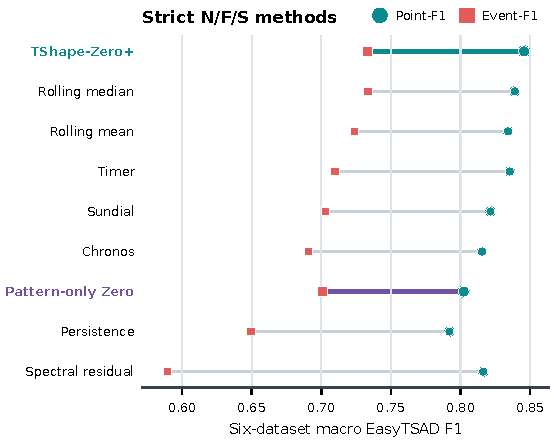
\includegraphics[width=\columnwidth]{figures/fig_strict_overall.pdf}
  \caption{Macro performance of directly deployable no-fit, frozen, and strict synthetic-only methods. Each segment connects a method's \efone{} (square) and \pfone{} (circle). Table~\ref{tab:all-easytsad} reports the non-residual per-dataset results; the public ledger retains access status for every method.}
  \label{fig:overall}
\end{figure}

Fig.~\ref{fig:overall} makes the central comparison readable without hiding the long table. Pattern-only TShape-Zero reaches \PatternMacroPoint{}/\PatternMacroEvent{} macro \pfone{}/\efone{}. Adding the guard raises the result to \FinalMacroPoint{}/\FinalMacroEvent{}, a gain of 0.044/0.032. TimesFM is the strongest official checkpoint on macro \pfone{} at 0.857 and obtains 0.733 macro \efone{}; \method{} is 0.012 lower on \pfone{} and effectively tied at the reported three-decimal \efone{} precision. Rolling median remains a serious deployment control at 0.839/0.734. Thus, the result supports a compact and inspectable TShape upgrade, not universal superiority.

The per-dataset cells expose complementary regimes. Among the ranked frozen/strict checkpoints, \method{} is strongest on Yahoo for both metrics and second on AIOPS and TODS \pfone{}, while the Pattern-only checkpoint is strongest on NAB. TimesFM leads AIOPS, TODS, and WSD and leads UCR \pfone{}; Timer leads UCR \efone{}. Some adapter rows obtain larger individual cells under different packaging or adaptation contracts, which is why their provenance remains explicit in the public ledger rather than being conflated with official frozen-checkpoint evidence. This heterogeneity is precisely why an out-of-the-box product must retain channel evidence and why average-only claims would be unsafe.

\textbf{Answer to RQ1.}
One strict \method{} checkpoint provides full six-dataset coverage and is competitive with checkpoints thousands of times larger. It substantially repairs Pattern-only TShape, but strong foundation and residual controls still win particular targets and metrics.

\subsection{RQ2: Pattern Bank Effectiveness}

\begin{figure}[t]
  \centering
  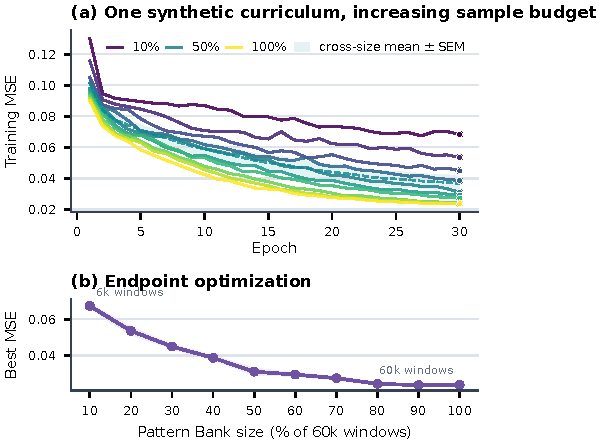
\includegraphics[width=\columnwidth]{figures/fig_strict_pattern_training.pdf}
  \caption{Pattern Bank optimization from 10\% to 100\%. (a) Training trajectories and their cross-size envelope. (b) Best training MSE against the nested number of generated windows. Every size uses the same generator mixture and seed.}
  \label{fig:pattern-training}
\end{figure}

\begin{figure}[t]
  \centering
  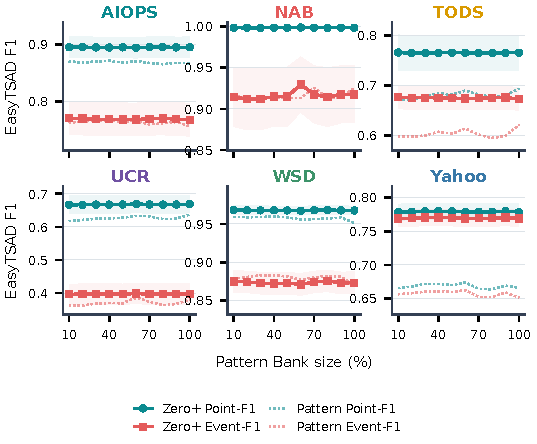
\includegraphics[width=\columnwidth]{figures/fig_strict_pattern_effect.pdf}
  \caption{Pattern Bank size sweep on all six datasets, arranged as two rows of three panels. Dotted curves are the neural Pattern-only channel; solid curves are the same checkpoints after the fixed Residual Guard. Every point is a full-series \pfone{} or \efone{} evaluation; labeled panel-specific ranges expose within-target change without implying cross-panel scale equality.}
  \label{fig:pattern-effect}
\end{figure}

The size sweep uses strict nested prefixes of one generated stream: 10\% contains 6,000 windows and each step adds 6,000 until the 60,000-window bank is complete. Generator identities, random seed, incident rate, optimizer, maximum epochs, and stopping rule remain fixed. Consequently, Fig.~\ref{fig:pattern-training} measures additional generated evidence rather than an order-dependent addition of hand-selected pattern families.

Training loss and target F1 answer different questions. More generated windows constrain continuation on the Pattern Bank, so optimization should improve or saturate. An unseen benchmark, however, is never consulted when choosing bank size; its F1 may fluctuate because additional synthetic variation can help one target and dilute another. Fig.~\ref{fig:pattern-effect} therefore reports every measured endpoint rather than smoothing the curve into artificial monotonicity. The 100\% checkpoint is the release model because it realizes the predeclared full-diversity curriculum, not because target labels selected a favorable fraction.

The measured curves make this boundary concrete. Best training MSE falls from 0.0674 with 6,000 windows to 0.0237 with 60,000, a 64.8\% reduction, and the slope visibly flattens after 48,000 windows. Across targets, Pattern-only macro \pfone{}/\efone{} starts at 0.797/0.696, reaches 0.804/0.703 at 60\%, and finishes at 0.802/0.701. The additional bank evidence is clearest on TODS (0.673 to 0.694 \pfone{}) and UCR (0.617 to 0.637), while already saturated or mismatched targets show smaller reversals. After the fixed guard, all ten checkpoints lie in the narrow 0.845--0.846 \pfone{} and 0.733--0.735 \efone{} bands. Thus the bank improves the learned synthetic objective and selected transfer regimes, while the guard converts target-specific fluctuations into a stable release envelope.

The six panels also separate learning from fallback behavior. A movement in a dotted curve is attributable to the checkpoint. A smaller movement in the corresponding solid curve means that the fixed guard absorbs neural instability; a larger movement means that newly learned shape evidence complements the guard. This distinction prevents the Pattern Bank claim from borrowing gains produced by residual channels.

\textbf{Answer to RQ2.}
The Pattern Bank supplies measurable zero-shot shape evidence under a benchmark-independent training contract. Increasing generated coverage sharply improves and then saturates the training objective, but target F1 is not guaranteed to be monotone. The fixed guard reduces the operational cost of that residual transfer variance; the 100\% release is selected by coverage policy, not target-label performance.

\subsection{RQ3: Residual Guard Effectiveness}

\begin{figure}[t]
  \centering
  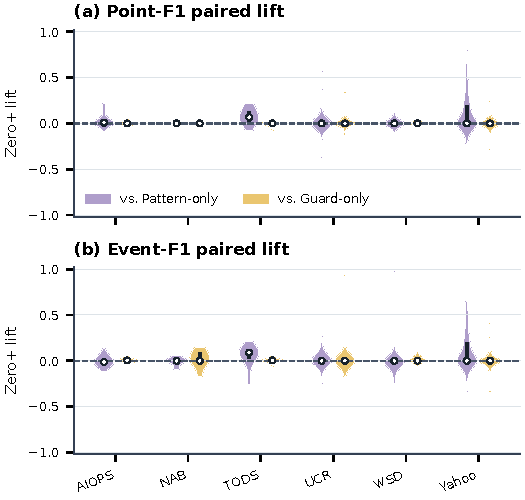
\includegraphics[width=\columnwidth]{figures/fig_strict_guard_violin.pdf}
  \caption{Paired series-level lift of \method{} over Pattern-only TShape (purple) and over the exactly matched residual-only guard (gold). Violin density, interquartile bar, and median expose both average repair and harmed series.}
  \label{fig:guard-violin}
\end{figure}

\begin{figure}[t]
  \centering
  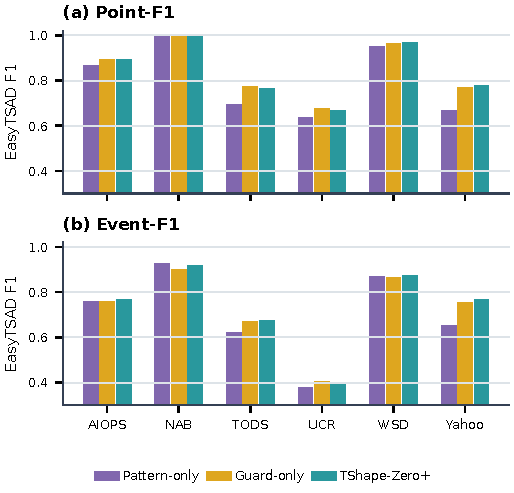
\includegraphics[width=\columnwidth]{figures/fig_strict_guard_bars.pdf}
  \caption{Dataset-level decomposition for Pattern-only, guard-only, and final \method{}. The neural comparison isolates repair; the matched-guard comparison isolates TShape's marginal contribution.}
  \label{fig:guard-bars}
\end{figure}

Figs.~\ref{fig:guard-violin} and~\ref{fig:guard-bars} separate algorithmic contribution from engineering protection. Relative to Pattern-only TShape, final fusion improves macro \pfone{} by 0.044 and macro \efone{} by 0.032. Point-F1 gains are positive with bootstrap intervals above zero on AIOPS, TODS, UCR, WSD, and Yahoo; Yahoo gains 0.113/0.118 in paired mean \pfone{}/\efone{}. NAB is already saturated and its small Event-F1 change is negative.

The stricter comparator is the guard itself. Guard-only obtains \GuardMacroPoint{}/\GuardMacroEvent{}, versus \FinalMacroPoint{}/\FinalMacroEvent{} for final fusion. Their macro \pfone{} values are effectively equal, while TShape adds 0.007 macro \efone{}. At series level, the Event-F1 intervals are positive on AIOPS, WSD, and Yahoo; UCR remains a failure boundary. This is a bounded but nonzero neural contribution: the guard supplies most of the reliability floor, while learned repeated-shape evidence improves selected event regimes.

\begin{table}[t]
\caption{Paired series-level repair effects. Cells are mean difference [bootstrap 95\% interval]. PB: strict Pattern-only TShape-Zero; G: matched residual-only guard.}
\label{tab:paired-effects}
\centering
\scriptsize
\setlength{\tabcolsep}{2.3pt}
\resizebox{\columnwidth}{!}{%
\begin{tabular}{lrrrr}
\toprule
Dataset & $\Delta$Point vs. PB & $\Delta$Event vs. PB & $\Delta$Point vs. G & $\Delta$Event vs. G \\
\midrule
AIOPS & +0.028 [+0.006,+0.053] & +0.011 [-0.019,+0.047] & +0.000 [-0.007,+0.007] & +0.009 [+0.002,+0.017] \\
NAB & -0.000 [-0.001,+0.000] & -0.008 [-0.035,+0.016] & +0.000 [-0.001,+0.002] & +0.016 [-0.040,+0.066] \\
TODS & +0.072 [+0.030,+0.115] & +0.052 [-0.009,+0.104] & -0.008 [-0.022,+0.002] & +0.004 [-0.010,+0.015] \\
UCR & +0.032 [+0.012,+0.053] & +0.016 [-0.006,+0.041] & -0.008 [-0.018,+0.003] & -0.008 [-0.033,+0.017] \\
WSD & +0.016 [+0.004,+0.033] & +0.005 [-0.016,+0.027] & +0.003 [+0.000,+0.006] & +0.009 [+0.002,+0.016] \\
Yahoo & +0.113 [+0.090,+0.136] & +0.118 [+0.095,+0.142] & +0.010 [-0.000,+0.020] & +0.015 [+0.003,+0.026] \\
\bottomrule
\end{tabular}}
\end{table}


\begin{figure}[t]
  \centering
  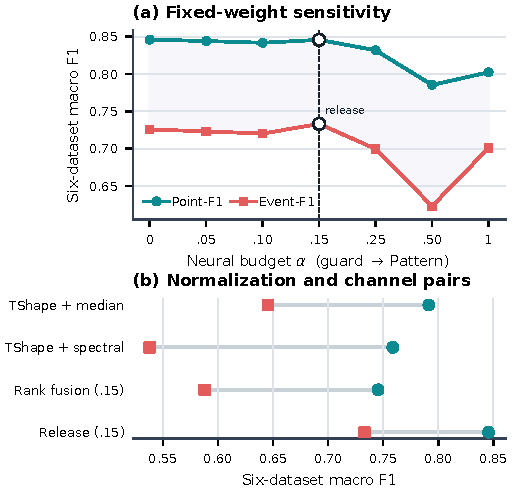
\includegraphics[width=\columnwidth]{figures/fig_strict_guard_ablation.pdf}
  \caption{Residual Guard ablations over six-dataset macro \pfone{} and \efone{}. The sweep varies neural budget $\alpha$, score normalization, and pairwise evidence channels while holding the strict Pattern checkpoint fixed.}
  \label{fig:guard-ablation}
\end{figure}

The ablation in Fig.~\ref{fig:guard-ablation} tests whether Eq.~\eqref{eq:fusion} is merely a renamed residual ensemble. The endpoints $\alpha=0$ and $\alpha=1$ are guard-only and Pattern-only. The release obtains \FinalMacroPoint{}/\FinalMacroEvent{} at $\alpha=0.15$; guard-only obtains \GuardMacroPoint{}/\GuardMacroEvent{}. Thus the guard is marginally higher in macro \pfone{}, while 0.15 is higher in macro \efone{}. Raising the neural budget to 0.50 reduces the scores to 0.785/0.623, showing why residual-first weighting is necessary. TShape+median and TShape+spectral reach only 0.792/0.645 and 0.759/0.538, so no single guard component explains the final result. Rank-normalized 0.15 fusion reaches 0.745/0.588, confirming that the documented min--max score contract is consequential. The release keeps $\alpha=0.15$ as a conservative, predeclared reliability budget; we do not relabel it as universally target-optimal.

\begin{figure}[t]
  \centering
  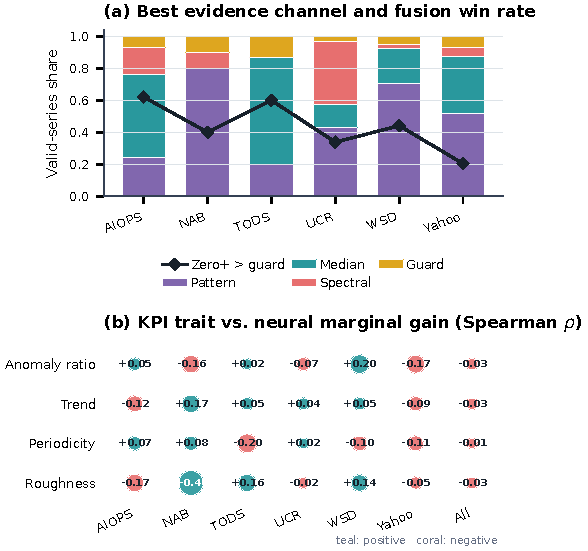
\includegraphics[width=\columnwidth]{figures/fig_strict_channel_attribution.pdf}
  \caption{EasyTSAD channel attribution over paired valid series. (a) Stacked bars identify the strongest individual evidence channel; diamonds show how often final fusion beats the exactly matched guard. (b) Bubble size and color encode the Spearman association between four unlabeled KPI traits and final fusion gain. This is a diagnostic, not a target-trained gate.}
  \label{fig:channel-attribution}
\end{figure}

Fig.~\ref{fig:channel-attribution} asks a stricter question than a favorable case study: can one explain when the neural channel adds value? Panel (a) compares Pattern-only TShape with median, spectral, and combined-guard evidence on every paired valid series, then reports the final fusion win rate against that same guard. Panel (b) relates the paired mean of Point-F1 and Event-F1 gains to anomaly ratio, trend, periodicity, and roughness. The traits are computed only after scores are frozen and are never used for checkpoint or weight selection. Their associations are descriptive rather than a learned target gate; weak or conflicting cells are themselves evidence that channel attribution should be returned to the operator instead of being replaced by an opaque universal routing rule.

\textbf{Answer to RQ3.}
The Residual Guard is responsible for most average robustness, and the paper states that fact directly. TShape remains useful where repeated local/global shape evidence improves event ranking beyond the matched guard, especially on AIOPS, WSD, and Yahoo; it is not indispensable on every KPI.

\subsection{RQ4: Effectiveness, Footprint, and Learned Behavior}

\begin{figure}[t]
  \centering
  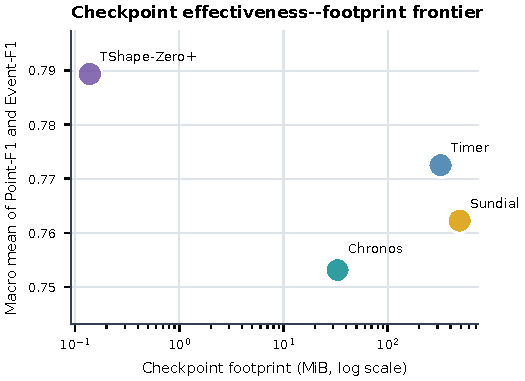
\includegraphics[width=\columnwidth]{figures/fig_strict_effectiveness_bubble.pdf}
  \caption{Effectiveness--distribution frontier for strict frozen checkpoints. Position is checkpoint footprint versus mean macro F1; bubble area encodes macro \efone{}. Upper left is preferable.}
  \label{fig:effectiveness}
\end{figure}

Fig.~\ref{fig:effectiveness} combines effectiveness with release cost. The \method{} checkpoint is 0.138 MiB, compared with 33.0 MiB for Chronos, 321.0 MiB for Timer, 489.6 MiB for Sundial, and 882.3 MiB for TimesFM. TimesFM's macro advantage is 0.012 \pfone{} and less than 0.001 \efone{}, while its distributed checkpoint is over 6,000 times larger. The final Pattern model trains in 128 seconds; dense stride-one inference over all 834 series and 15.1 million aligned points takes 291 seconds on the study MPS device. Footprint is not latency, but it directly affects artifact transfer, cold start, versioning, and edge placement. Runtime metadata remain available separately so the bubble plot does not pretend that heterogeneous foundation-model hardware timings are architecture-only effects.

\begin{figure}[t]
  \centering
  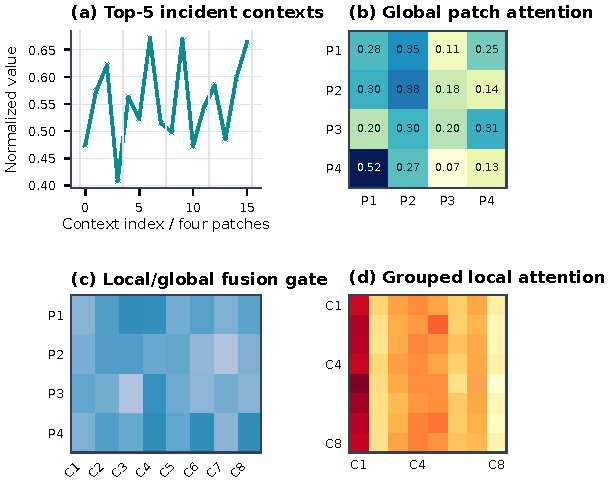
\includegraphics[width=\columnwidth]{figures/fig_strict_attention.pdf}
  \caption{Mechanism trace for the frozen checkpoint on top-ranked points from the real deployment case: incident contexts, global patch attention, local/global fusion gate, and grouped local attention. Attention is descriptive evidence, not a causal explanation.}
  \label{fig:attention}
\end{figure}

Fig.~\ref{fig:attention} verifies that the released neural channel is active rather than a dead weight in the residual ensemble. On the top-ranked incident contexts, global attention connects nonadjacent patches while the fusion gate varies across patches and channels. The local map emphasizes repeated within-patch structure. These traces establish input-dependent execution and support debugging; they do not prove that an attention coefficient caused a correct alarm.

\textbf{Answer to RQ4.}
\method{} occupies a favorable compact-checkpoint region and exposes internal and residual evidence through one scorer. Its efficiency claim is distribution footprint and full-series executability, not an unsupported universal latency claim.

\subsection{Threats to Validity}

\textbf{Construct validity.}
Point adjustment can reward long events~\cite{kim2022rigorous}. We use it because the original TShape claim uses EasyTSAD, pair it with logarithmic event weighting, and apply the exact same implementation to every score stream. Both metrics select thresholds with labels and therefore evaluate score separability, not an online alarm policy.

\textbf{Internal validity.}
One fixed seed makes the full sweep reproducible and computationally tractable but cannot quantify optimizer-seed variance. Series-level bootstrap intervals quantify target heterogeneity only. Official foundation checkpoints and no-fit controls are ranked separately from adapters, source adaptation, and target-context diagnostics. The Pattern Bank checkpoint metadata states that no benchmark values or labels enter weight fitting.

\textbf{Baseline validity.}
Four foundation rows use released checkpoints directly. Many anomaly families lack an equivalent frozen univariate interface; their X rows are executable family adapters, not claims of official reproduction. Unknown overlap between public benchmarks and foundation pretraining corpora may advantage those checkpoints. TimeMoE is omitted under the predeclared runtime rule rather than completed on a biased subset.

\textbf{External and deployment validity.}
The six families span industrial Internet-service KPIs, Web-service monitoring, public cloud streams, controlled anomalies, and rare-event archives, but remain univariate historical benchmarks. Proprietary multivariate and causal streaming settings may differ. Per-history score normalization uses the complete batch; online deployment requires a rolling or source-calibrated transform. The web case is illustrative and selected after the aggregate protocol was frozen, so it is not used as independent effectiveness evidence.
